\newpage % Rozdziały zaczynamy od nowej strony.
\section{Przegląd literaratury}

Przegląd literatury związanej z rozwiązywanym problemem. 

W pracy~\cite{he2016deep} opisano ....
W~\cite{liu2022convnet} zaproponowano nowatorską architekturę....
Przykładowy obraz~\ref{fig:convnext}.

\begin{figure}[h]
    \centering
    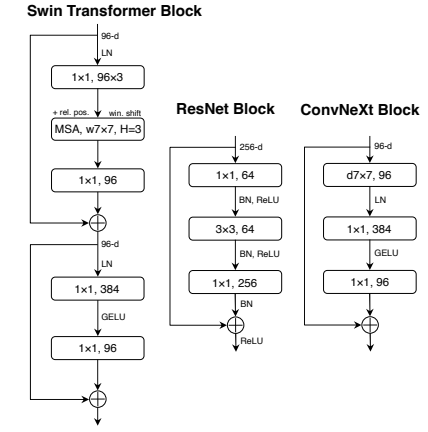
\includegraphics[width=0.5\textwidth]{rysunki/convnext_block.png}
    \caption{Porównanie bloków rezydualnych wykorzystywanych w sieci Swin Transformer, ResNet i ConvNeXt.}
    \label{fig:convnext}
\end{figure}
